% Energy level diagrams - illustrating Hund's rule
% Author: Henri Menke
\documentclass[tikz, border=10pt]{standalone}
\usepackage{siunitx}
\usetikzlibrary{shapes.callouts,decorations.pathmorphing}
\tikzset{
  level/.style   = { ultra thick },
  connect/.style = { dashed, red },
  notice/.style  = { draw, rectangle callout, callout relative pointer={#1} },
  label/.style   = { text width=2cm },
  trans/.style   = { dashed, blue },
  snake it/.style= { decorate, decoration=snake }
}
\begin{document}
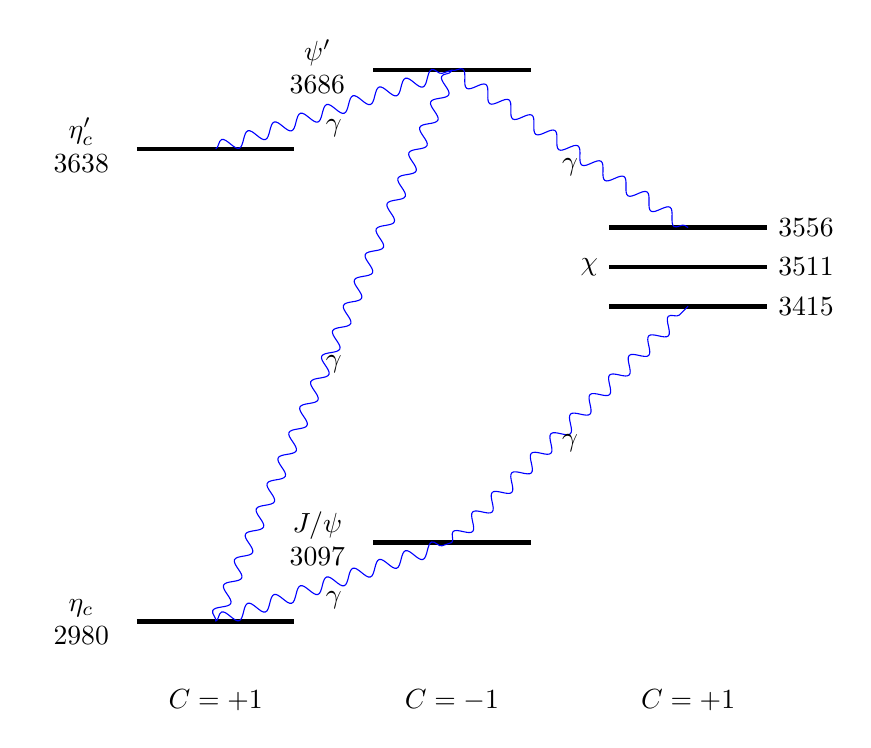
\begin{tikzpicture}
    \draw[level] node[left] at (0,0) {\begin{tabular}{c}\( \eta_c \)\\2980\end{tabular}} (0,0) -- (2,0);
    \draw[level] node[left] at (0,6) {\begin{tabular}{c}\( \eta_c' \)\\3638\end{tabular}} (0,6) -- (2,6);

    \draw[level] node[left] at (3,1) {\begin{tabular}{c}\( J/\psi \)\\3097\end{tabular}} (3,1) -- (5,1);
    \draw[level] node[left] at (3,7) {\begin{tabular}{c}\( \psi' \)\\3686\end{tabular}} (3,7) -- (5,7);

    \draw[level] (6,4) -- (8,4) node[right] at (8,4) {3415};
    \draw[level] node[left] at (6,4.5) {\( \chi \)} (6,4.5) -- (8,4.5) node[right] at (8,4.5) {3511};
    \draw[level] (6,5) -- (8,5) node[right] at (8,5) {3556};

    \draw[draw=blue, snake it] (1,0) -- node[below] {\( \gamma \)} (4,1);
    \draw[draw=blue, snake it] (1,0) -- node[below] {\( \gamma \)} (4,7);
    \draw[draw=blue, snake it] (1,6) -- node[below] {\( \gamma \)} (4,7);
    \draw[draw=blue, snake it] (4,1) -- node[below] {\( \gamma \)} (7,4);
    \draw[draw=blue, snake it] (4,7) -- node[below] {\( \gamma \)} (7,5);

    \draw node at (1,-1) {\( C = +1 \)};
    \draw node at (4,-1) {\( C = -1 \)};
    \draw node at (7,-1) {\( C = +1 \)};


  %% Draw labels
  %\node[label] at (4,5.5)  {Spin-spin interaction};
  %\node[label] at (7,5.5)  {Orbit-orbit interaction};
  %\node[label] at (10,5.5) {Spin-orbit interaction};
%
  %% Draw annotations
  %\node[notice={(0.5,0.5)}, text width=1.5cm] at (2,-3) {Hunds rule \# 1};
  %\node[notice={(0,1)}] at (4,-4) {Why is triplet lower};
  %\node[notice={(0.7,0.7)}, text width=3cm] at (6,-5)
%    {Why is higher angular momentum state lower energy?};
  %\node[notice={(-0.9,0.9)}, text width=1.5cm] at (9,-5) {Hunds rule \# 2};
  %\node[notice={(-0.2,1.6)}, text width=3cm] at (11,-6.5)
%    {Why is low total angular momentum state lower in energy?};
  %\node[notice={(-0.5,0.5)}, text width=1.5cm] at (12,-5) {Hunds rule \# 3};
\end{tikzpicture}
\end{document}
